\section{Results}
\label{sec:results}

Averages are over the five Liars' Bench datasets, which we call the \emph{five-dataset mean}, and every
result is at layer~40 unless stated.

\subsection{The problem}
\label{sec:problem-measured}

Liars' Bench evaluates three linear probes on Llama-3.3-70B-Instruct \cite{kretschmar2025liars}: the
Mean Probe, whose recipe our base probe follows, the Follow-Up Probe, and the Upper-Bound Probe, which
is trained with privileged labelled examples from the same five datasets and so is a ceiling, not a
fair rival. Averaged over the five datasets, they reach AUROCs of \V{lb-mean-auroc-avg},
\V{lb-followup-auroc-avg} and \V{lb-upper-auroc-avg}. On \hpkr{} the Mean Probe catches none of the
lies, and the Follow-Up Probe's recall of 0.37 comes with a false-positive rate of 0.84.

\emph{Ranking is not detection.} Our base probe ranks \hpkr{} at an AUROC of \V{bp-auroc-hpkr-L40},
yet its balanced accuracy is \V{bp-balacc-hpkr-L40}, because it flags none of \hpkr's \V{ndec-hpkr}
lies and none of its honest responses. At layer~20, the layer the benchmark's probes read, it inverts
on \hpkr, at \V{bp-auroc-hpkr-L20}, close to the published 0.12. The published persona contrast, which
uses no labels, also inverts there: built from our bank, it reads \V{zs-dec-hpkr-L20} at layer~20, and
\V{zs-dec-hpkr-L40} at layer~40, inside the random band, which reaches \V{th-rand-hpkr-L40} on \hpkr.
Because whether a response denies knowledge ranks \hpkr{} at \V{th-hk-denial-auroc} on its own, a
detector that reads a denial of knowledge as honest will rank \hpkr{} backwards, and one that reads it
as deceptive will rank it well without reading the lie.

\subsection{Persona contrasts at 70B}
\label{sec:zeroshot}

\emph{Supervised probes transfer poorly.} The probe on raw activations averages \V{diag-base-L40} AUROC
on its own dataset and \V{off-base-L40} on the other five; with \hpkr{} removed the off-diagonal mean is
still \V{offx-base-L40}. The base probe averages \V{bp-auroc-lb-L40} and inverts on insider trading
(\V{bp-auroc-it-L40}). Training it on the model's own lies raises its five-dataset mean by
\V{th-aisi-gain-L40} [\V{th-aisi-gain-lo-L40}, \V{th-aisi-gain-hi-L40}] but does not close the gap to
the extended contrast. The published persona method's three components transfer at
\V{off-pcthree-L40}, below the raw probe; at 70B they beat it only at layer~20 (\V{off-pcthree-L20}
against \V{off-base-L20}). Three components of the extended contrast's 25 roles do better, at
\V{off-extpcthree-L40}, but the single extended direction does better still, at \V{off-ext-L40}.

\emph{The persona result.} The extended contrast ranks lies across datasets better than any supervised
design we tested. Scored zero-shot, with no training and no labels from the benchmark, it reaches a
five-dataset mean AUROC of \V{zs-ext-lb-L40}, against \V{lb-mean-auroc-avg} for the benchmark's Mean
Probe, \V{lb-followup-auroc-avg} for its Follow-Up Probe and \V{bp-auroc-lb-L40} for our base probe at
the same layer. On the benchmark's main metric, balanced accuracy at the Alpaca threshold, it reaches
\V{op-ext-balacc-L40}, against \V{lb-mean-balacc-avg} for the Mean Probe and \V{lb-followup-balacc-avg}
for the Follow-Up Probe. Across the 16-layer sweep it is above the base probe at every layer.

\emph{The roles, not the widening.} The extended contrast differs from the published one only by the ten
knowledge-denial roles, and its mean over the six datasets is \V{th-kd-gain-L40} higher, most of all
on \hpkr. The unified contrast widens the published contrast by the same operation, with the
sycophantic roles in place of the knowledge-denial roles, and it does not help. Averaged over the 16
layers it transfers at \V{th-uni-off-mean}, below the \V{th-dec-off-mean} of the published contrast it
widens and far below the \V{th-ext-off-mean} of the extended contrast, and its \hpkr{} AUROC is above
0.5 at only \V{th-uni-above-chance-n} of the \V{th-uni-layers} layers. Widening the bank is therefore
not what changes \hpkr; adding roles that deny knowledge is.

\subsection{Persona directions read the wording}
\label{sec:hpkr-tests}

\emph{What the knowledge-denial contrast flags.} It is the only detector whose balanced accuracy on
\hpkr{} leaves 0.5, at \V{op-den-balacc-hpkr-L40}, zero-shot. This is not evidence that it tells a
feigned denial from a sincere one. Its threshold flags \V{th-k-deight-flag-lies-L40}\% of \hpkr's lies
and \V{th-k-deight-flag-hden-L40}\% of its honest denials, the answers of a model that truly does not
know, while it flags \V{th-k-deight-flag-hclaims-L40}\% of the honest answers that claim knowledge. Its
balanced accuracy is high only because honest denials are \V{th-k-den-honest} of \hpkr's
\V{th-honest-hpkr} honest answers. The extended contrast ranks \hpkr{} almost as well
(\V{op-ext-auroc-hpkr-L40}), but its threshold flags no \hpkr{} lie.

\emph{With the words held fixed.} On the identical-text slice the published, knowledge-denial and
extended contrasts read \V{th-k-dfive-ident-L40}, \V{th-k-deight-ident-L40} and
\V{th-k-dnine-ident-L40}, all inside the random band of \V{th-k-ident-band-L40}, and from layer~32 to
layer~72 no persona direction's identical-text AUROC exceeds \V{th-k-depth-persona-ident-max}, about the
height of the band (\cref{fig:k-hpkr}). On the denials slice the knowledge-denial contrast, the
contrast built for \hpkr, is the weakest.

\emph{Gender-Secret.} Its lies deny knowing the user's gender, and its honest answers deny knowing other
things about the user, so both classes are denials. Read through the fine-tuned model, every persona
direction is at chance: the knowledge-denial contrast scores \V{th-gs-den-L40}, and rebuilding it from
the bank's rollouts read through the fine-tune raises it at best to \V{th-gs-ft-best}. The three tests
agree. On \hpkr{} the persona directions' signal goes with the words of a denial, and where the words
are controlled none of them reads the lie.

\begin{figure*}[t]
\centering
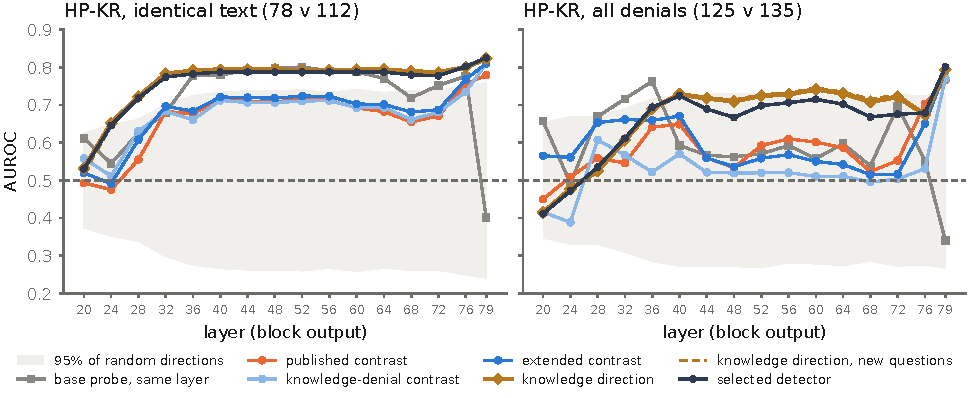
\includegraphics{fig_knowledge_hpkr.pdf}
\caption{\hpkr's wording-controlled slices across 16 layers; grey: 95\% of random directions.}
\label{fig:k-hpkr}
\end{figure*}

\subsection{The knowledge direction}
\label{sec:k-results}

\Cref{tab:knowledge} gives the knowledge direction beside the extended contrast, the selected detector,
the benchmark's Mean Probe and the base probe trained at layer~40, on every set.

\begin{table}[t]
\centering
\footnotesize
\setlength{\tabcolsep}{3.2pt}
\caption{AUROC at layer 40. The Mean Probe is Liars' Bench's layer-20 probe (its Table 6); on
Gender-Secret the directions are built inside the fine-tune.}
\label{tab:knowledge}
\resizebox{\columnwidth}{!}{% Generated by make_thesis_assets.py
\begin{tabular}{@{}l ccc ccc@{}}
\toprule
 & \multicolumn{2}{c}{Trained on RepE} & \multicolumn{3}{c}{Zero-shot, layer 40} \\
\cmidrule(lr){2-3}\cmidrule(lr){4-6}
Evaluation set & Mean Probe & \shortstack{base probe,\\layer 40} & \shortstack{extended\\contrast} & \shortstack{knowledge\\direction} & \shortstack{selected\\detector} \\
\midrule
CG & 1.00 & 0.972 & 0.912 & 0.641 & 0.865 \\
HP-C & 0.41 & 0.675 & 0.712 & 0.830 & 0.820 \\
HP-KR & 0.12 & 0.936 & 0.912 & 0.865 & 0.909 \\
IT & 0.93 & 0.338 & 0.980 & 0.881 & 0.975 \\
ID & 0.95 & 0.971 & 0.978 & 0.906 & 0.962 \\
Mean of the five & 0.682 & 0.778 & 0.899 & 0.825 & 0.906 \\
\midrule
\hpkr, identical text & n/a & 0.779 & 0.721 & 0.793 & 0.787 \\
\hpkr, denials & n/a & 0.593 & 0.670 & 0.728 & 0.724 \\
Gender-Secret & 0.45 & 0.524 & 0.547 & 0.861 & 0.841 \\
\bottomrule
\end{tabular}
}
\end{table}

\emph{\hpkr{} with the words held fixed.} On the identical-text slice the knowledge direction reads
\V{th-k-k-ident-L40} [\V{th-k-ident-lo-L40}, \V{th-k-ident-hi-L40}], above the random band of
\V{th-k-ident-band-L40}. With its wording component removed it reads \V{th-k-ident-nowording-L40}, so
on this slice it does not use the words. From layer~32 to layer~72 it stays between
\V{th-k-depth-ident-min} and \V{th-k-depth-ident-max}, above the random band at
\V{th-k-depth-ident-above} of the \V{th-k-depth-n} layers, and the direction rebuilt from the
replication questions lies on the same curve (\cref{fig:k-hpkr}). The selected detector follows it, at
\V{th-k-ninek-ident-L40}. The base probe trained at the same layer is the one detector
that keeps up with the knowledge direction on this slice, but it is trained on RepE's labels and fails
on insider trading and on Gender-Secret. On the full \hpkr{} the knowledge direction reads
\V{th-k-full-L40}, but that number rests on the words: with its wording component removed it falls to
\V{th-k-full-nowording-L40}, which is why we credit it, like the persona directions, only with the
slices.

\emph{Gender-Secret, read through the fine-tune.} Gender-Secret is the test the knowledge direction was
not designed on (\cref{fig:k-gs}). Built inside the fine-tune, it reads \V{th-k-gs-ft-kft-L40}
[\V{th-k-gs-ft-kft-lo-L40}, \V{th-k-gs-ft-kft-hi-L40}], above a random band of
\V{th-k-gs-ft-band-L40}. The extended contrast, rebuilt the same way, stays at chance
(\V{th-k-gs-ft-dnineft-L40}), and the selected detector reads \V{th-k-gs-ft-ninekft-L40}; the
benchmark's Mean Probe reads \V{th-lb-mean-auroc-gs}. The same transcripts read by the base model give
the knowledge direction only \V{th-k-gs-base-kft-L40}, so the signal is in the fine-tuned model's state,
not in the text, and it is not the adapter's own mean shift: removing that shift from the direction
leaves \V{th-k-gs-nooffset-L40}. Two cautions remain. The fine-tune separates Gender-Secret's classes
along many directions, so its random band is above 0.80 and the knowledge direction clears it by a few
hundredths. And the classes differ in topic as well as in knowledge: the lies concern the user's gender
and the honest answers other attributes.

\begin{figure*}[t]
\centering
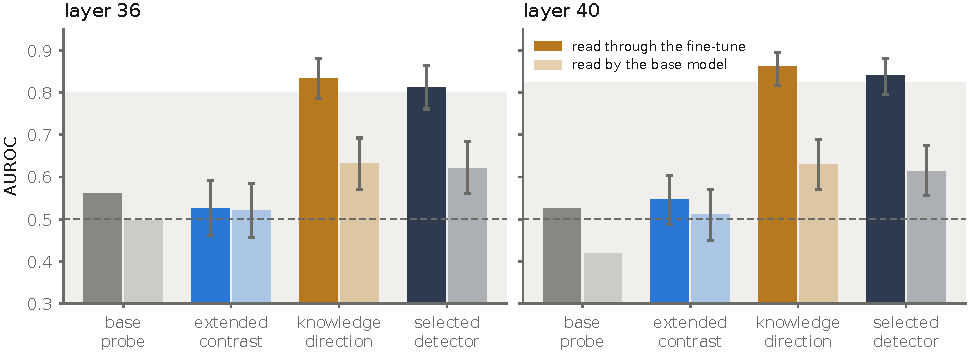
\includegraphics{fig_knowledge_gs.pdf}
\caption{Gender-Secret read through the fine-tune (dark) and by the base model (light); grey: 95\% of
random directions.}
\label{fig:k-gs}
\end{figure*}

\emph{The five datasets.} On the five Liars' Bench datasets the knowledge direction alone averages
\V{th-k-k-mean-L40}, below the extended contrast's \V{th-k-dnine-mean-L40}. It is strongest where the
persona directions are weakest: on \hpc{} it reads \V{th-k-k-auroc-hpc-L40} against the extended
contrast's \V{th-k-dnine-auroc-hpc-L40}. Added to the extended contrast, it lifts \hpc{} to
\V{th-k-ninek-auroc-hpc-L40} and costs a little elsewhere, most on CG (\V{th-k-ninek-auroc-cg-L40}). On
Soft-Trigger the base model's read of the same transcripts scores as high as the fine-tune's, because in
the released data the trigger itself predicts the label, so we report it as consistent with the
knowledge direction, not as evidence for it.

\subsection{Transfer across datasets}
\label{sec:transfer}

\Cref{fig:transfer} shows the train-one-test-all matrices of the probe on raw activations and of the
selected detector. The raw probe fits each training set but transfers unevenly: 6 of its 30
off-diagonal cells fall below chance, and the probe trained on RepE scores insider trading at 0.274.
Each row of the selected detector's matrix is constant off the diagonal by construction, since all six
training sets agree on the sign. Its mean off-diagonal AUROC is \V{th-k-ninek-off-L40}, against
\V{off-base-L40} for the raw probe and level with the extended contrast (\V{off-ext-L40}); without
\hpkr{} it is \V{th-k-ninek-offx-L40}. A probe on raw activations trained on the other five datasets
pooled, which needs all their labels, averages \V{th-pool-auroc}; with \hpkr{} left out it is level
with the extended contrast (\V{th-pool-offx} against \V{offx-ext-L40}), so the extended contrast's lead
over supervision that has seen many kinds of lie rests on \hpkr.

\begin{figure*}[t]
\centering
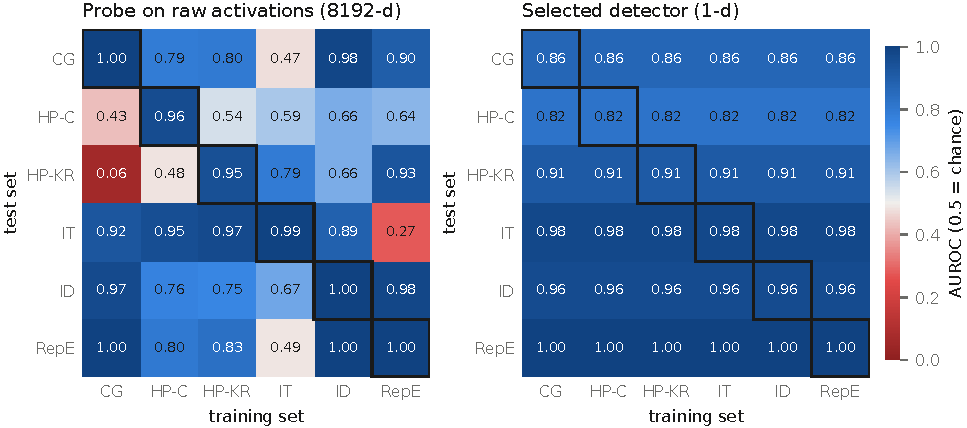
\includegraphics{fig_transfer_selected.pdf}
\caption{Train-one-test-all AUROC at layer 40 for the probe on raw activations (left) and the selected
detector (right).}
\label{fig:transfer}
\end{figure*}

\emph{Across depth.} \Cref{fig:selected-depth} follows the selected detector's transfer over the
\V{depth-n} layers of the sweep. It stays ahead of the published and unified contrasts and of the raw
probe at every layer, by at least \V{th-k-ninek-depth-lead-min} (at
layer~\V{th-k-ninek-depth-lead-min-layer}). The lead is thinnest where the knowledge direction is weak,
and averaged over the 16 layers the selected detector reaches \V{th-k-ninek-depth-off-mean}, below the
extended contrast's \V{th-ext-off-mean}: the extended contrast alone degrades less with depth. The raw
probe stays between \V{th-k-ninek-depth-probe-min} and \V{th-k-ninek-depth-probe-max} at every depth,
so its weak transfer is not a layer-40 accident.

\begin{figure*}[t]
\centering
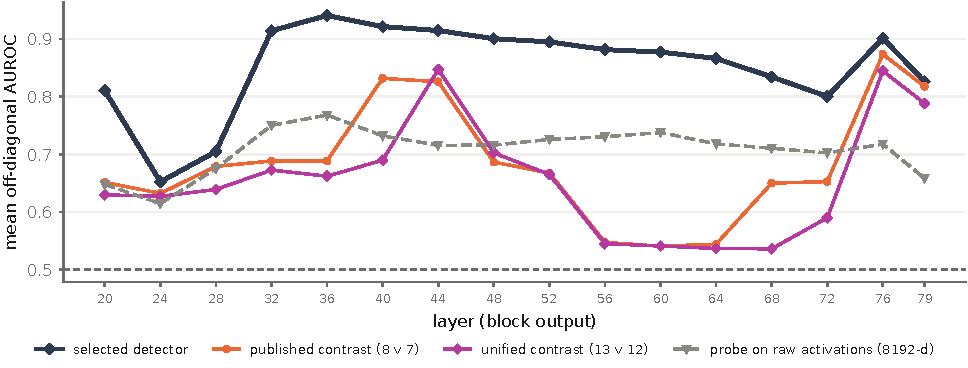
\includegraphics{fig_selected_depth.pdf}
\caption{Transfer of the selected detector across 16 layers, against two persona contrasts and the
probe on raw activations.}
\label{fig:selected-depth}
\end{figure*}

\subsection{Selection}
\label{sec:selection}

\Cref{tab:selection} places the designs side by side; BA is balanced accuracy at the Alpaca threshold.
No design wins every column. On transfer the selected detector and the extended contrast are level at
the top. On the five-dataset mean the selected detector is highest, at \V{th-k-ninek-mean-L40}, but only
\V{th-pair-ninek-dnine-mean-L40} above the extended contrast, a paired difference whose interval
includes zero ([\V{th-pair-ninek-dnine-mean-lo-L40}, \V{th-pair-ninek-dnine-mean-hi-L40}]). On the
identical-text slice, the one column where the words cannot help, the knowledge direction leads, and
every persona contrast is inside the random band. The knowledge-denial contrast has the highest
balanced accuracy, but on \hpkr{} it comes from flagging denials; the base probe ranks the full \hpkr{}
best, but flags none of its lies and inverts on insider trading.

\begin{table*}[t]
\centering
\footnotesize
\caption{The designs at layer 40 against the evaluation criteria.}
\label{tab:selection}
% Generated by make_thesis_assets.py
\begin{tabular}{@{}l l cc cc cc@{}}
\toprule
& & \multicolumn{2}{c}{Transfer AUROC} & \multicolumn{2}{c}{Five-dataset mean} & \multicolumn{2}{c}{\hpkr{} AUROC} \\
\cmidrule(lr){3-4}\cmidrule(lr){5-6}\cmidrule(lr){7-8}
Design & Labels & all six & excl.\ \hpkr{} & AUROC & BA & all & identical \\
\midrule
Probe on raw activations & one dataset & 0.732 & 0.758 & n/a & n/a & n/a & n/a \\
Base probe (RepE) & RepE & n/a & n/a & 0.778 & 0.626 & 0.936 & 0.779 \\
Base probe, own lies (AISI) & AISI & n/a & n/a & 0.878 & 0.630 & 0.935 & 0.686 \\
Persona method, extended PCs ($k=3$) & one dataset & 0.866 & 0.867 & n/a & n/a & n/a & n/a \\
Published contrast & none & 0.832 & 0.880 & 0.798 & 0.675 & 0.593 & 0.715 \\
Sycophancy contrast & none & 0.663 & 0.936 & 0.770 & 0.601 & 0.167 & 0.686 \\
Unified contrast & none & 0.690 & 0.919 & 0.795 & 0.655 & 0.381 & 0.707 \\
Knowledge-denial contrast & none & 0.912 & 0.910 & 0.894 & 0.725 & 0.919 & 0.712 \\
Extended contrast & none & 0.916 & 0.917 & 0.899 & 0.694 & 0.912 & 0.721 \\
\midrule
Knowledge direction & none & 0.823 & 0.815 & 0.825 & 0.553 & 0.865 & 0.793 \\
Published contrast + knowledge direction & none & n/a & n/a & 0.879 & 0.646 & 0.854 & 0.789 \\
Selected detector (extended + knowledge) & none & 0.922 & 0.924 & 0.906 & 0.701 & 0.909 & 0.787 \\
\bottomrule
\end{tabular}

\end{table*}

We therefore select one design, the extended contrast plus the knowledge direction at layer~40. It
needs no labels, costs one inner product per response, and is the only design at or near the top on
transfer, the five-dataset mean, the identical-text slice and Gender-Secret at once. Its case over the
extended contrast does not rest on transfer or the average, where the two are level, but on the data
where the words are controlled: it gains \V{th-pair-ninek-dnine-ident-L40}
[\V{th-pair-ninek-dnine-ident-lo-L40}, \V{th-pair-ninek-dnine-ident-hi-L40}] on the identical-text
slice and \V{th-k-gs-gain-L40} on Gender-Secret, at the price of small losses on CG, instructed
deception and insider trading.

\subsection{Robustness and operating points}
\label{sec:k-robustness}

\emph{The knowledge direction's robustness.} Resampling its 120 questions moves its identical-text
AUROC by no more than \V{th-k-boot-ident-width}. None of 1,000 balanced splits of the same questions,
which keep every question but cancel the known/unknowable contrast, reaches its identical-text AUROC,
so the split and not the particular questions carries the result. Built from the replication questions
written afterwards, the direction has a cosine of \V{th-k-rep-cos-L40} with the original and met all
\V{th-k-rep-criteria} criteria fixed before its reads were scored. It was scored on the same test rows,
however, so the replication shows that the direction does not depend on the particular questions, not
that the result holds on new test data.

\emph{The tail.} At strict thresholds detection is weaker than ranking. With the cutoff set to flag 1\%
of a dataset's own honest answers, the extended contrast catches \V{th-k-op-dnine-1-L40} of the lies on
average, the selected detector \V{th-k-op-ninek-1-L40}, the same-layer base probe
\V{th-k-op-probe-1-L40} and the knowledge direction \V{th-k-op-k-1-L40}; at 10\% they catch
\V{th-k-op-dnine-10-L40}, \V{th-k-op-ninek-10-L40}, \V{th-k-op-probe-10-L40} and \V{th-k-op-k-10-L40}.
Adding the knowledge direction costs detection in the tail. Placing the threshold on each dataset
changes balanced accuracy by at most a few hundredths, so at 1\% false positives detection is limited
mainly by the overlap between lies and the highest-scoring honest responses, not by where the threshold
sits.

\subsection{Steering}
\label{sec:steering}

\Cref{tab:steering} gives the change in disclosure at $c = \pm 0.3$ over the \V{th-steer-n} scenarios.
Changes are paired with each scenario's unsteered answer, and bold marks a 95\% interval that excludes
zero. Adding the extended contrast cuts disclosure from \V{th-steer-base} to \V{th-steer-ext-plus}, a
paired change of \V{th-steer-ext-plus-change} [\V{th-steer-ext-plus-lo}, \V{th-steer-ext-plus-hi}]. The
published contrast does the same (\V{th-steer-dec-plus-change}), and two random directions at the same
strength do not. The steered answers adopt the deceptive personas' manner rather than merely omitting
the fact: the estate agent's termites become ``the usual, uh, summer pests'', which a random direction
at the same strength still admits. Subtracting the extended contrast raises disclosure to
\V{th-steer-ext-minus}, a borderline gain. The base probe moves disclosure by only
\V{th-steer-base-plus-change} [\V{th-steer-base-plus-lo}, \V{th-steer-base-plus-hi}]: a direction
fitted to separate labelled examples need not be one the model acts on, whereas the difference of two
persona means, which describes how the model behaves in role, is. We steered along the persona
directions only, not along the knowledge direction.

\begin{table*}[t]
\centering
\small
\caption{Disclosure of the hidden fact under steering, over \V{th-steer-n} scenarios.}
\label{tab:steering}
\begin{tabular}{lcccc}
\toprule
 & \multicolumn{2}{c}{honest side ($c=-0.3$)} & \multicolumn{2}{c}{deceptive side ($c=+0.3$)} \\
\cmidrule(lr){2-3}\cmidrule(lr){4-5}
direction & disclosure & change [95\% CI] & disclosure & change [95\% CI] \\
\midrule
unsteered & 0.48 & -- & 0.48 & -- \\
extended contrast (12 v 13) & 0.61 & $+0.13$ [0.00, $+0.26$] & 0.20 & {\boldmath$-0.28$} [$-0.41$, $-0.13$] \\
published contrast (8 v 7) & 0.57 & $+0.09$ [$-0.06$, $+0.24$] & 0.20 & {\boldmath$-0.28$} [$-0.41$, $-0.15$] \\
base probe (trained on RepE) & 0.50 & $+0.02$ [$-0.11$, $+0.15$] & 0.39 & $-0.09$ [$-0.22$, $+0.04$] \\
random direction 1 & 0.43 & $-0.06$ [$-0.17$, $+0.04$] & 0.48 & 0.00 [$-0.09$, $+0.09$] \\
random direction 2 & 0.46 & $-0.02$ [$-0.09$, $+0.06$] & 0.52 & $+0.04$ [$-0.11$, $+0.19$] \\
\bottomrule
\end{tabular}

\end{table*}
